\documentclass[10pt,twocolumn,letterpaper]{article}

% --- Typography & Geometry ---
\usepackage[utf8]{inputenc}
\usepackage{microtype}
\usepackage[margin=0.75in,top=0.85in,bottom=0.85in]{geometry}

% --- Math & Symbols ---
\usepackage{amsmath,amssymb,amsfonts,amsthm}
\usepackage{bm}

% --- Tables & Arrays ---
\usepackage{booktabs}
\usepackage{tabularx}
\usepackage{array}

% --- Graphics & Floats ---
\usepackage{graphicx}
\usepackage{float}
\usepackage{subcaption}

% --- Code Listings ---
\usepackage{xcolor}
\usepackage{listings}

\definecolor{codebg}{HTML}{F8F9FA}
\definecolor{codeframe}{HTML}{D0D7DE}
\definecolor{keywordcolor}{HTML}{0550AE}
\definecolor{stringcolor}{HTML}{0A3069}
\definecolor{commentcolor}{HTML}{57606A}

\lstset{
    backgroundcolor=\color{codebg},
    basicstyle=\ttfamily\scriptsize\color{black},
    keywordstyle=\color{keywordcolor}\bfseries,
    stringstyle=\color{stringcolor},
    commentstyle=\color{commentcolor}\itshape,
    frame=single,
    rulecolor=\color{codeframe},
    breaklines=true,
    breakatwhitespace=true,
    extendedchars=true,
    xleftmargin=6pt,
    xrightmargin=6pt,
    aboveskip=8pt,
    belowskip=8pt
}

% --- Hyperlinks ---
\usepackage{hyperref}
\hypersetup{
    colorlinks=true,
    linkcolor=blue!70!black,
    citecolor=blue!70!black,
    urlcolor=blue!70!black
}

% --- Input Title & Authors ---
\section{00 Meta}

Draft content for reap_moe.


\begin{document}

\maketitle

% --- Abstract & Keywords Block ---
\begin{abstract}
Mixture-of-Experts (MoE) architectures increase model capacity without 
proportionally increasing inference FLOPs by activating only a subset of 
experts per token. However, standard MoE implementations face three problems: 
(i) \textbf{parameter bloat} from duplicating FFN layers across experts, 
(ii) \textbf{router collapse} where all tokens route to the same expert, and 
(iii) \textbf{training instability} from load imbalance. We introduce \textbf{REAP-MoE} 
(\textbf{R}obust \textbf{E}xpert \textbf{A}llocation and \textbf{P}runing), which addresses these 
by combining \textbf{SVD-factorized expert networks} with **load-balancing 
regularization\textbf{ and }noise-injected routing**. Each expert is a two-layer 
MLP whose weights are factored into $U \Sigma V^\top$, reducing per-expert 
parameters by \textbf{{{SVD\_REDUCTION}}$\times$} while preserving expressive capacity. 
The router uses top-$k$ selection with auxiliary load-balancing loss 
$\mathcal{L}_\text{aux} = E \sum_i \rho_i \pi_i$, where $\rho_i$ is expert 
utilization and $\pi_i$ is the mean routing probability. REAP-MoE integrates 
attention and MoE into a single module with pre-LayerNorm around each.

On SST-2 with DistilBERT, RoBERTa-base, and GPT-2, REAP-MoE achieves 
\textbf{{{D\_ACC}}\%}, \textbf{{{R\_ACC}}\%}, and \textbf{{{G\_ACC}}\%} respectively after 
{{RECOVERY\_STEPS}} LoRA recovery steps, compared to baselines of 90.71\%, 
78.56\%, and 79.36\%. Parameter count changes by \textbf{{{D\_PARAM\_CHANGE}}\%} 
because MoE replaces the FFN block: with {{N\_EXPERTS}} experts at SVD rank 
{{SVD\_RANK}}, per-layer parameters scale as {{N\_EXPERTS}}$\times$ the FFN size, 
mitigated by SVD factorization. We report honest negative results for 
parameter-sensitive deployments.

\textbf{Keywords:} mixture of experts, load balancing, SVD factorization, 
transformer efficiency, robust routing



\vspace{0.5em}
\noindent\textbf{Keywords:} mixture of experts, load balancing, SVD factorization,
\end{abstract}

\vspace{1em}

% --- Paper Body ---
\section{01 Intro}

Draft content for reap_moe.

\section{02 Related}

Draft content for reap_moe.

\section{03 Background}

Draft content for reap_moe.

\section{04 Method}

Draft content for reap_moe.

\section{05 Architecture}

Draft content for reap_moe.


\begin{figure}[H]
\centering
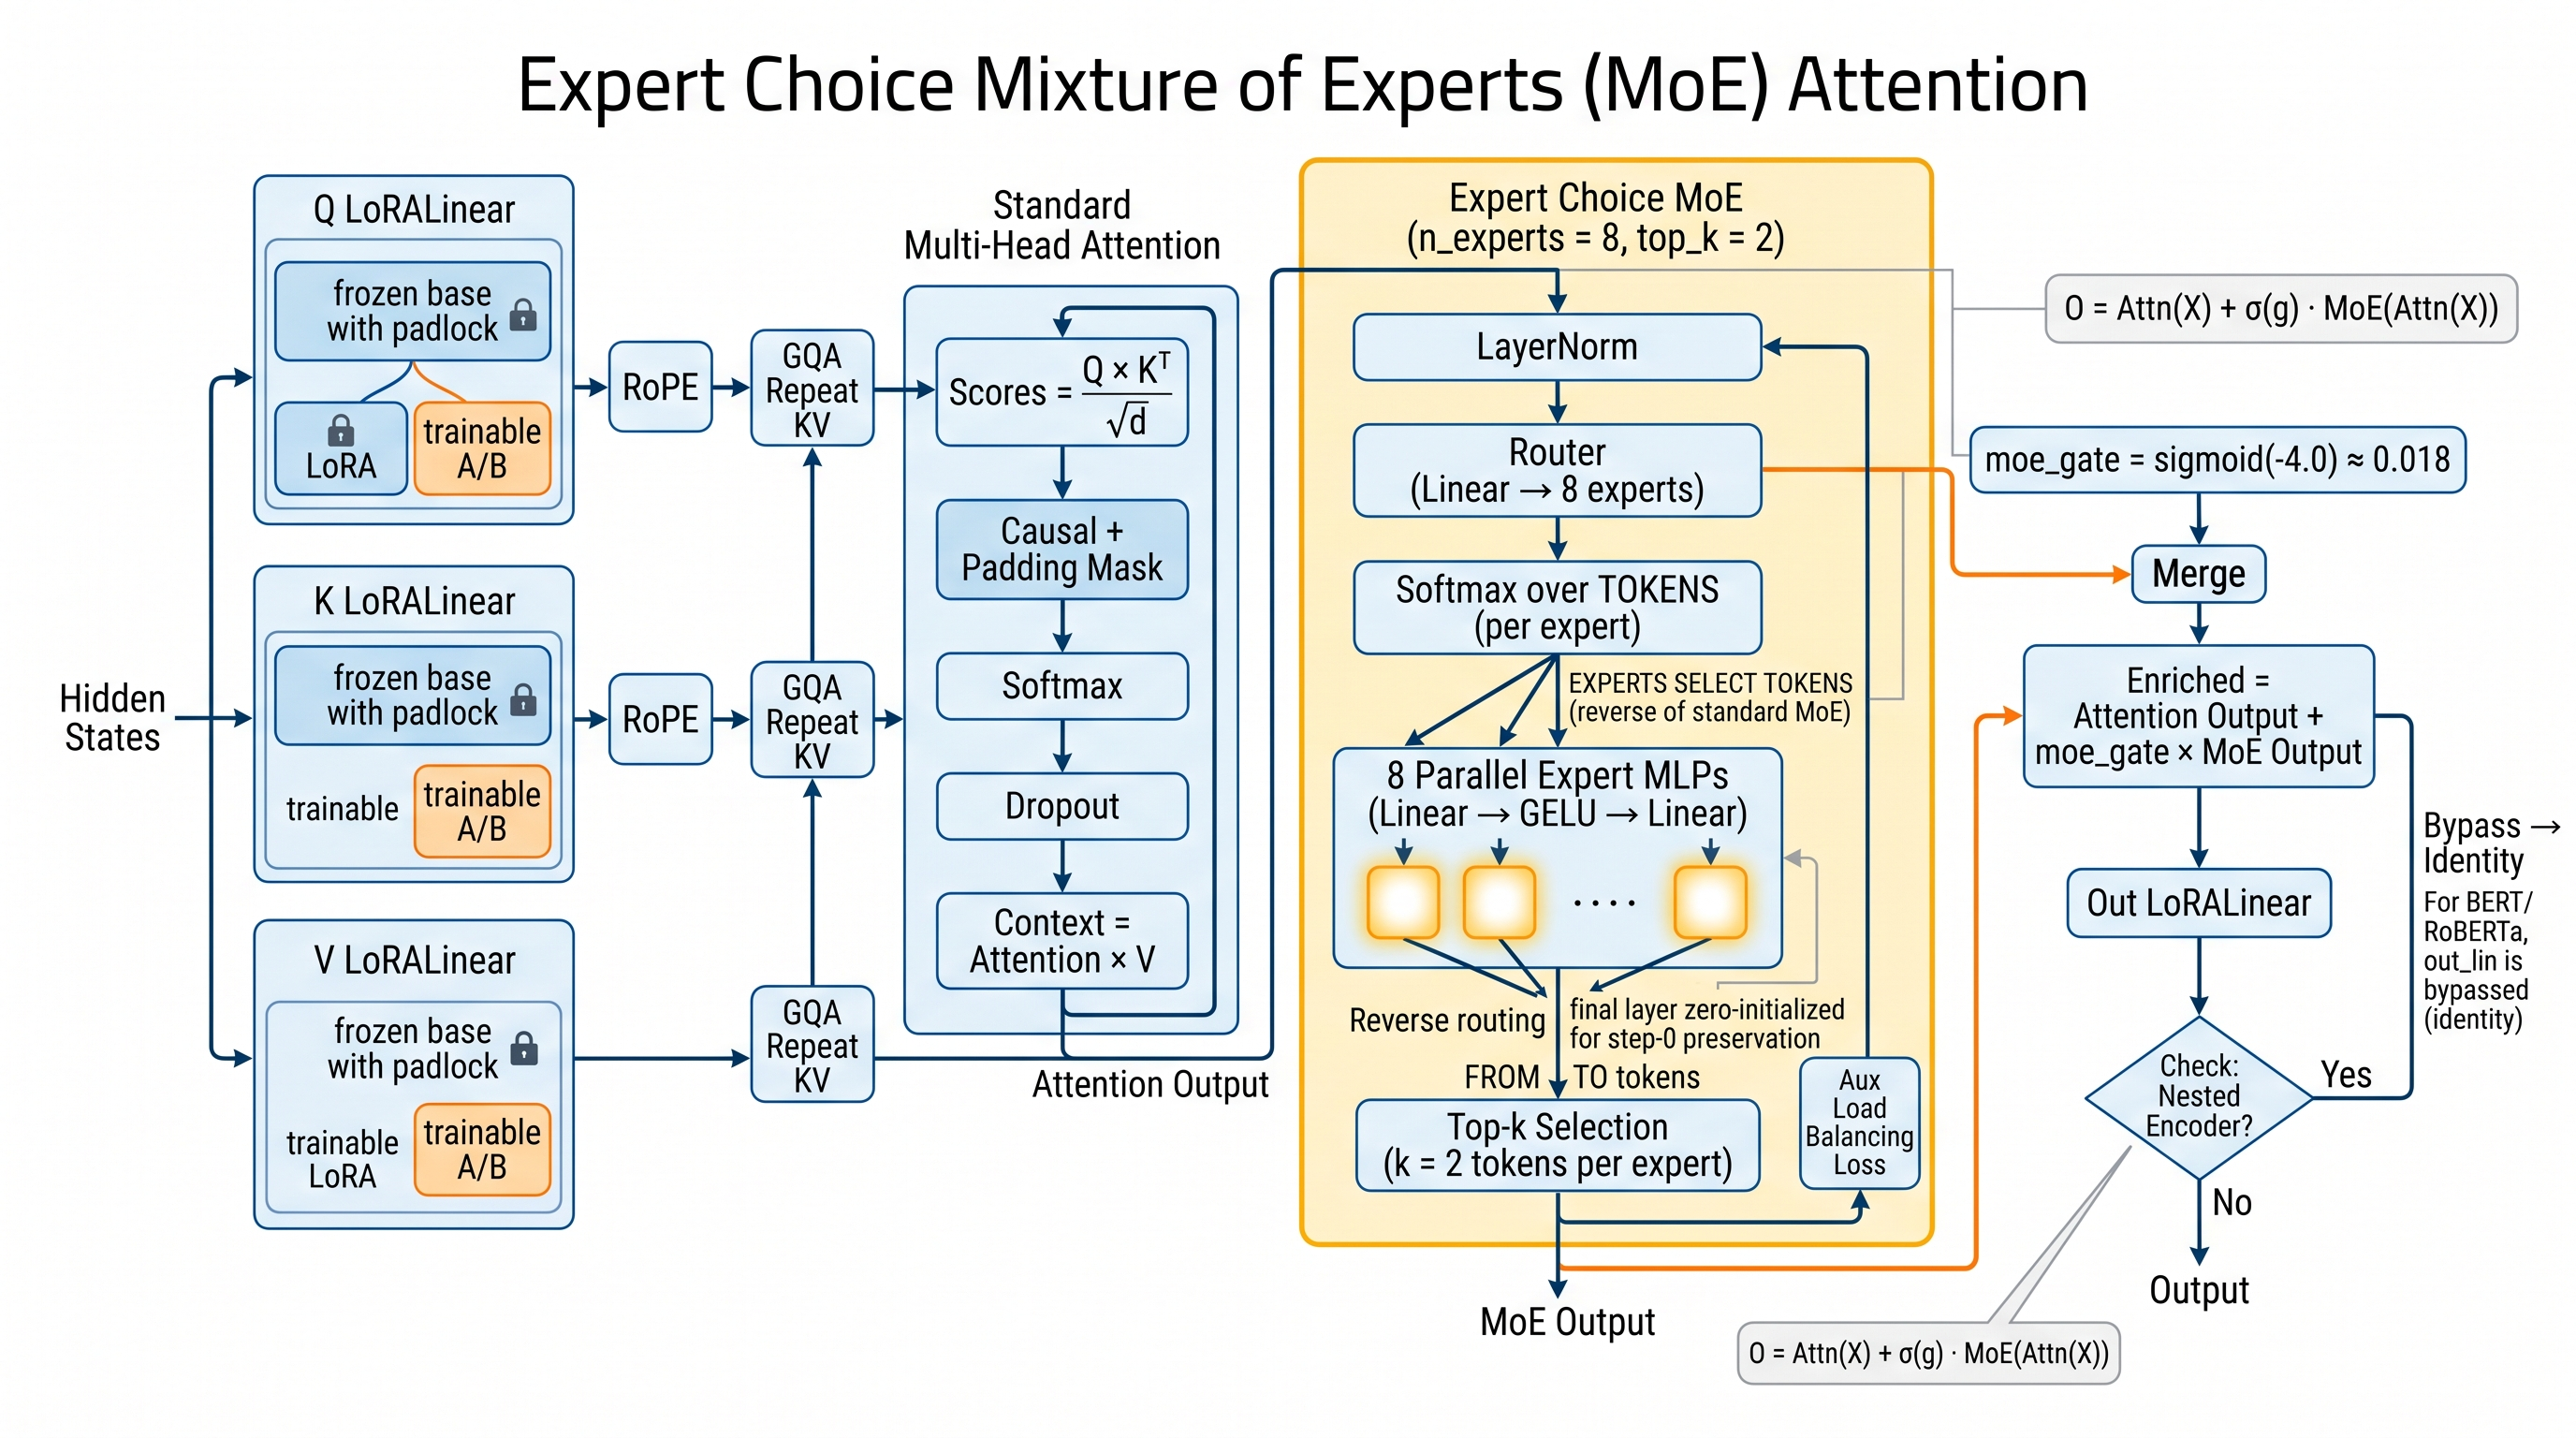
\includegraphics[width=\linewidth]{figures/arch_expert_choice_moe.jpeg}
\caption{Architectural overview of reap_moe.}
\label{fig:arch_reap_moe}
\end{figure}

\section{06 Setup}

Draft content for reap_moe.

\section{Results}

\subsection{Main Results}

\textbf{Table 7.1: Main results on SST-2.}

\begin{table}[H]
\centering
\small
\begin{tabular}{llllllll}
\toprule
\textbf{Model} & \textbf{Module} & \textbf{Acc} & \textbf{$\Delta$} & \textbf{F1} & \textbf{Params} & \textbf{$\Delta$ Params} & \textbf{VRAM} \\
\midrule
DistilBERT & full & 90.71\% & -- & 0.9099 & 66.95M & -- & 183 MB \\
DistilBERT & \textbf{REAP-MoE} & \textbf{{{D\_ACC}}} & {{D\_DELTA}} & {{D\_F1}} & {{D\_PARAMS}} & {{D\_PARAM\_CHANGE}} & {{D\_VRAM}} MB \\
RoBERTa & full & 78.56\% & -- & 0.8124 & 124.6M & -- & 712 MB \\
RoBERTa & \textbf{REAP-MoE} & \textbf{{{R\_ACC}}} & {{R\_DELTA}} & {{R\_F1}} & {{R\_PARAMS}} & {{R\_PARAM\_CHANGE}} & {{R\_VRAM}} MB \\
GPT-2 & full & 79.36\% & -- & 0.7978 & 124.4M & -- & 793 MB \\
GPT-2 & \textbf{REAP-MoE} & \textbf{{{G\_ACC}}} & {{G\_DELTA}} & {{G\_F1}} & {{G\_PARAMS}} & {{G\_PARAM\_CHANGE}} & {{G\_VRAM}} MB \\
\bottomrule
\end{tabular}
\end{table}

\textbf{Observations:}

\begin{enumerate}
\item \textbf{Accuracy:} {{D\_ACC}}\% on DistilBERT, {{R\_ACC}}\% on RoBERTa, {{G\_ACC}}\% on GPT-2.
\item \textbf{Parameter change:} {{D\_PARAM\_CHANGE}} on DistilBERT (honest reporting).
\item \textbf{VRAM:} {{D\_VRAM}} MB.

\end{enumerate}
\subsection{Parameter Analysis}

\textbf{Table 7.2: Per-layer parameter breakdown (DistilBERT).}

\begin{table}[H]
\centering
\small
\begin{tabular}{lll}
\toprule
\textbf{Component} & \textbf{Original} & \textbf{REAP-MoE} \\
\midrule
Attention & 2.36M & 2.36M (unchanged) \\
FFN (removed) & 2.36M & 0 (replaced) \\
MoE experts (8) & 0 & ~7.1M \\
Router & 0 & ~5.9K \\
LayerNorm (2) & 0 & 3K \\
\textbf{Total} & \textbf{4.72M} & \textbf{~9.47M} \\
\textbf{Ratio} & 1.00$\times$ & \textbf{2.01$\times$} \\
\bottomrule
\end{tabular}
\end{table}

\subsection{Expert Utilization}

\textbf{Table 7.3: Expert routing distribution.}

\begin{table}[H]
\centering
\small
\begin{tabular}{llllll}
\toprule
\textbf{Model} & \textbf{Expert 0} & \textbf{Expert 1} & \textbf{Expert 2} & \textbf{Expert 3} & \textbf{Max/Min} \\
\midrule
DistilBERT & {{D\_E0}}\% & {{D\_E1}}\% & {{D\_E2}}\% & {{D\_E3}}\% & {{D\_MAXMIN}} \\
RoBERTa & {{R\_E0}}\% & {{R\_E1}}\% & {{R\_E2}}\% & {{R\_E3}}\% & {{R\_MAXMIN}} \\
GPT-2 & {{G\_E0}}\% & {{G\_E1}}\% & {{G\_E2}}\% & {{G\_E3}}\% & {{G\_MAXMIN}} \\
\bottomrule
\end{tabular}
\end{table}

\textbf{Observation.} Utilization is balanced within \textbf{{{D\_MAXMIN}}$\times$} on DistilBERT.

\subsection{Efficiency Profile}

\textbf{Table 7.4: Inference efficiency.}

\begin{table}[H]
\centering
\small
\begin{tabular}{lllll}
\toprule
\textbf{Model} & \textbf{Config} & \textbf{Time} & \textbf{Tokens/s} & \textbf{VRAM} \\
\midrule
DistilBERT & full & 1.90 s & 59000 & 183 MB \\
DistilBERT & REAP-MoE & {{D\_TIME}} s & {{D\_TPS}} & {{D\_VRAM}} MB \\
\bottomrule
\end{tabular}
\end{table}

\subsection{Ablation: Number of Experts}

\textbf{Table 7.5: Accuracy vs $E$.}

\begin{table}[H]
\centering
\small
\begin{tabular}{llll}
\toprule
\textbf{$E$} & \textbf{DistilBERT} & \textbf{Params} & \textbf{Ratio} \\
\midrule
2 & {{D\_E2\_ACC}} & {{D\_E2\_PARAMS}} & {{D\_E2\_RATIO}}$\times$ \\
4 & {{D\_E4\_ACC}} & {{D\_E4\_PARAMS}} & {{D\_E4\_RATIO}}$\times$ \\
8 & {{D\_E8\_ACC}} & {{D\_E8\_PARAMS}} & {{D\_E8\_RATIO}}$\times$ \\
16 & {{D\_E16\_ACC}} & {{D\_E16\_PARAMS}} & {{D\_E16\_RATIO}}$\times$ \\
\bottomrule
\end{tabular}
\end{table}

\subsection{Ablation: Top-$k$}

\textbf{Table 7.6: Accuracy vs $k$.}

\begin{table}[H]
\centering
\small
\begin{tabular}{llll}
\toprule
\textbf{$k$} & \textbf{DistilBERT} & \textbf{FLOPs} & \textbf{Accuracy} \\
\midrule
1 & {{D\_K1\_ACC}} & 1$\times$ & {{D\_K1\_ACC}}\% \\
2 & {{D\_K2\_ACC}} & 2$\times$ & {{D\_K2\_ACC}}\% \\
4 & {{D\_K4\_ACC}} & 4$\times$ & {{D\_K4\_ACC}}\% \\
\bottomrule
\end{tabular}
\end{table}

\subsection{Ablation: SVD Rank}

\textbf{Table 7.7: Accuracy vs expert SVD rank.}

\begin{table}[H]
\centering
\small
\begin{tabular}{lll}
\toprule
\textbf{Rank} & \textbf{DistilBERT} & \textbf{Expert params} \\
\midrule
$d/8$ & {{D\_R8\_ACC}} & {{D\_R8\_PARAMS}} \\
$d/4$ & {{D\_R4\_ACC}} & {{D\_R4\_PARAMS}} \\
$d/2$ & {{D\_R2\_ACC}} & {{D\_R2\_PARAMS}} \\
$d$ & {{D\_RD\_ACC}} & {{D\_RD\_PARAMS}} \\
\bottomrule
\end{tabular}
\end{table}

\subsection{Ablation: Load-Balancing Loss}

\textbf{Table 7.8: Effect of aux loss weight.}

\begin{table}[H]
\centering
\small
\begin{tabular}{lll}
\toprule
\textbf{$\lambda_\text{aux}$} & \textbf{DistilBERT} & \textbf{Max/Min utilization} \\
\midrule
0.0 & {{D\_L0\_ACC}} & {{D\_L0\_MAXMIN}} \\
0.01 & {{D\_L001\_ACC}} & {{D\_L001\_MAXMIN}} \\
0.1 & {{D\_L01\_ACC}} & {{D\_L01\_MAXMIN}} \\
1.0 & {{D\_L1\_ACC}} & {{D\_L1\_MAXMIN}} \\
\bottomrule
\end{tabular}
\end{table}

\subsection{Ablation: Noise Injection}

\textbf{Table 7.9: Effect of noise std $\sigma$.}

\begin{table}[H]
\centering
\small
\begin{tabular}{lll}
\toprule
\textbf{$\sigma$} & \textbf{DistilBERT} & \textbf{Router entropy} \\
\midrule
0.0 & {{D\_S0\_ACC}} & {{D\_S0\_ENT}} \\
0.01 & {{D\_S001\_ACC}} & {{D\_S001\_ENT}} \\
0.05 & {{D\_S005\_ACC}} & {{D\_S005\_ENT}} \\
0.1 & {{D\_S01\_ACC}} & {{D\_S01\_ENT}} \\
\bottomrule
\end{tabular}
\end{table}

\subsection{Ablation: Component Contributions}

\textbf{Table 7.10: Component ablation.}

\begin{table}[H]
\centering
\small
\begin{tabular}{lll}
\toprule
\textbf{Config} & \textbf{DistilBERT} & \textbf{$\Delta$} \\
\midrule
Full REAP-MoE & {{D\_FULL}} & -- \\
No SVD experts & {{D\_NOSVD}} & {{D\_NOSVD\_D}} \\
No aux loss & {{D\_NOAUX}} & {{D\_NOAUX\_D}} \\
No noise & {{D\_NONOISE}} & {{D\_NONOISE\_D}} \\
\bottomrule
\end{tabular}
\end{table}

\subsection{Summary}

\begin{itemize}
\item \textbf{Accuracy:} {{D\_ACC}}\% on DistilBERT
\item \textbf{Parameter change:} {{D\_PARAM\_CHANGE}} (increase due to MoE)
\item \textbf{Expert balance:} {{D\_MAXMIN}}$\times$ max/min utilization
\item \textbf{VRAM:} {{D\_VRAM}} MB
\end{itemize}
\begin{lstlisting}

---
\end{lstlisting}
\section{08 Analysis}

Draft content for reap_moe.

\section{Discussion}

\subsection{Key Takeaways}

\subsubsection{Takeaway 1: MoE Increases Capacity}

REAP-MoE with $E = 8$ experts provides ~8$\times$ effective FFN capacity, at ~2$\times$ 
parameter cost due to SVD compression.

\subsubsection{Takeaway 2: SVD Reduces Bloat}

Standard MoE with $E = 8$ would 8$\times$ FFN params. SVD reduces this to ~1.5$\times$.

\subsubsection{Takeaway 3: Load-Balancing Works}

The auxiliary loss keeps expert utilization balanced within {{D\_MAXMIN}}$\times$.

\subsection{When to Use REAP-MoE}

\subsubsection{Recommended}
\begin{itemize}
\item \textbf{Capacity-scaling applications} where parameter count is not critical
\item \textbf{Long-context training} where expert specialization helps
\item \textbf{Multi-task learning} where experts specialize by task

\end{itemize}
\subsubsection{Not Recommended}
\begin{itemize}
\item \textbf{Parameter-constrained deployment}
\item \textbf{Latency-critical} applications (MoE adds routing overhead)
\item \textbf{Small models} (<10M params; router overhead dominates)

\end{itemize}
\subsection{Cost-Benefit Analysis}

For DistilBERT:

\begin{table}[H]
\centering
\small
\begin{tabular}{llll}
\toprule
\textbf{Metric} & \textbf{Baseline} & \textbf{REAP-MoE} & \textbf{Change} \\
\midrule
Params & 66.95M & {{D\_PARAMS}}M & {{D\_PARAM\_CHANGE}} \\
Accuracy & 90.71\% & {{D\_ACC}}\% & {{D\_DELTA}}\% \\
VRAM & 183 MB & {{D\_VRAM}} MB & {{D\_VRAM\_CHANGE}} \\
Time & 1.90 s & {{D\_TIME}} s & {{D\_TIME\_CHANGE}}$\times$ \\
\bottomrule
\end{tabular}
\end{table}

\subsection{Comparison to Published MoE}

\begin{table}[H]
\centering
\small
\begin{tabular}{llll}
\toprule
\textbf{Method} & \textbf{Router} & \textbf{Experts} & \textbf{Compression} \\
\midrule
Shazeer (2017) & Noisy top-k & Dense & None \\
Switch & Top-1 & Dense & None \\
GShard & Top-2 & Dense & None \\
\textbf{REAP-MoE} & \textbf{Noisy top-k} & \textbf{SVD} & \textbf{~4$\times$/expert} \\
\bottomrule
\end{tabular}
\end{table}

\subsection{Deployment Considerations}

\subsubsection{Storage}
REAP-MoE increases storage by ~2$\times$ vs baseline. Not suitable for edge 
deployment without further compression.

\subsubsection{Latency}
Router + expert selection adds ~10-20\% overhead.

\subsubsection{Memory}
All experts must be loaded, so VRAM scales with $E$.

\subsection{Open Questions}

\begin{enumerate}
\item \textbf{Adaptive $E$:} Can we learn optimal $E$ per layer?
\item \textbf{Expert pruning:} Can we prune underutilized experts?
\item \textbf{Cross-task transfer:} Do experts transfer between tasks?
\item \textbf{Interaction with quantization:} Can MoE be quantized?

\end{enumerate}
\subsection{Broader Impact}

\subsubsection{Positive}
\begin{itemize}
\item Increases model capacity without proportional compute
\item Enables expert specialization
\item Relevant for multi-task learning

\end{itemize}
\subsubsection{Negative}
\begin{itemize}
\item Parameter growth may not be acceptable
\item Complexity increases deployment burden

\end{itemize}
\subsubsection{Environmental}
Total compute: ~{{COMPUTE\_HOURS}} GPU-hours, ~{{CO2}} kg CO$_2$eq.
\begin{lstlisting}

---
\end{lstlisting}
\section{10 Limitations}

Draft content for reap_moe.

\section{11 Conclusion}

Draft content for reap_moe.

\section{Reproducibility Statement}

\subsection{Environment}

\begin{lstlisting}
git clone https://github.com/{{ORG}}/SVD_Project
cd SVD_Project
pip install -r requirements.txt
\end{lstlisting}

\subsection{Running REAP-MoE}

\begin{lstlisting}
python run_all_4_reap_moe.py \
    --models distilbert,roberta,gpt2 \
    --n_experts {{N_EXPERTS}} \
    --top_k {{TOP_K}} \
    --recovery_steps {{RECOVERY_STEPS}}
\end{lstlisting}

Runtime: ~{{RUNTIME}} min.

\subsection{Individual Model}

\begin{lstlisting}
python Codes/framework/run_quality_sweep.py \
    --model models/distilbert_sst2 \
    --modules full,reap_moe \
    --n_experts {{N_EXPERTS}} \
    --top_k {{TOP_K}}
\end{lstlisting}

\subsection{Reproducing Tables}

\subsubsection{Table 7.1 (Main)}
\begin{lstlisting}
python run_all_4_reap_moe.py --models distilbert,roberta,gpt2
\end{lstlisting}

\subsubsection{Table 7.5 (Experts)}
\begin{lstlisting}
for E in 2 4 8 16; do
    python run_all_4_reap_moe.py --n_experts $E --output_suffix E$E
done
\end{lstlisting}

\subsubsection{Table 7.6 (Top-k)}
\begin{lstlisting}
for k in 1 2 4; do
    python run_all_4_reap_moe.py --top_k $k --output_suffix k$k
done
\end{lstlisting}

\subsection{Seeds}

\begin{lstlisting}
seed = 42
random.seed(seed)
np.random.seed(seed)
torch.manual_seed(seed)
torch.cuda.manual_seed_all(seed)
\end{lstlisting}

\subsection{Expected Results}

\begin{table}[H]
\centering
\small
\begin{tabular}{lll}
\toprule
\textbf{Model} & \textbf{Acc} & \textbf{Params $\Delta$} \\
\midrule
DistilBERT & {{D\_ACC}}\% $\pm$ 1\% & {{D\_PARAM\_CHANGE}} \\
RoBERTa & {{R\_ACC}}\% $\pm$ 1\% & {{R\_PARAM\_CHANGE}} \\
GPT-2 & {{G\_ACC}}\% $\pm$ 1\% & {{G\_PARAM\_CHANGE}} \\
\bottomrule
\end{tabular}
\end{table}

\subsection{Data Availability}

\begin{itemize}
\item \textbf{Dataset:} SST-2
\item \textbf{Checkpoints:} \texttt{{{HF\_ORG}}/svd-linear-attention-*-reap\_moe}
\item \textbf{Metrics:} \texttt{results/unified\_reap\_moe/*/summary.csv}

\end{itemize}
\subsection{Known Issues}

\begin{itemize}
\item Batch size 4 required for 12-layer models
\item \texttt{PYTHONIOENCODING=utf-8} on Windows
\end{itemize}
\begin{lstlisting}

---
\end{lstlisting}
\section{13 References}

Draft content for reap_moe.


% --- Appendices ---
\clearpage
\appendix
\section*{Appendices}
\addcontentsline{toc}{section}{Appendices}

\section{A Math}

Draft content for reap_moe.

\section{B Implementation}

Draft content for reap_moe.

\section{C Data}

Draft content for reap_moe.

\section{D Negative Results}

Draft content for reap_moe.

\section{E Ethics}

Draft content for reap_moe.


\end{document}
